% -*- latex -*-
%%%%%%%%%%%%%%%%%%%%%%%%%%%%%%%%%%%%%%%%%%%%%%%%%%%%%%%%%%%%%%%%
%%%%%%%%%%%%%%%%%%%%%%%%%%%%%%%%%%%%%%%%%%%%%%%%%%%%%%%%%%%%%%%%
%%%%
%%%% This text file is part of the source of 
%%%% `Introduction to High-Performance Scientific Computing'
%%%% by Victor Eijkhout, copyright 2012-2022
%%%%
%%%% This book is distributed under a Creative Commons Attribution 3.0
%%%% Unported (CC BY 3.0) license and made possible by funding from
%%%% The Saylor Foundation \url{http://www.saylor.org}.
%%%%
%%%% blas.tex: tutorial on BLAS, LAPACK, SCALAPACK
%%%%
%%%%%%%%%%%%%%%%%%%%%%%%%%%%%%%%%%%%%%%%%%%%%%%%%%%%%%%%%%%%%%%%
%%%%%%%%%%%%%%%%%%%%%%%%%%%%%%%%%%%%%%%%%%%%%%%%%%%%%%%%%%%%%%%%


In this section we will discuss libraries for dense linear
algebra operations.

Dense linear algebra, that is linear algebra on matrices that are
stored as two-dimensional arrays (as opposed to sparse linear algebra;
see section~\HPSCref{sec:sparse}, as well as the
tutorial on PETSc~\PCSEref{part:petsc}) has been standardized for a
considerable time. The basic operations are defined by the three
levels of \indexac{BLAS}:
\begin{itemize}
\item Level~1 defines vector operations that are characterized by a
  single loop~\cite{Lawson:blas}.
\item Level~2 defines matrix vector operations, both explicit such as
  the matrix-vector product, and implicit such as the solution of
  triangular systems~\cite{BLAS2}.
\item Level~3 defines matrix-matrix operations, most notably the
  matrix-matrix product~\cite{BLAS3}.
\end{itemize}
The name `BLAS' suggests a certain amount of generality, but the
original authors were clear~\cite{Lawson:blas} that these subprograms
only covered dense linear algebra. Attempts to standardize sparse
operations have never met with equal success.

Based on these building blocks libraries have been built that tackle
the more sophisticated problems such as solving linear systems, or
computing eigenvalues or singular values.
\indexterm{Linpack}\footnote{The linear system solver from this
  package later became the \indextermbus{Linpack}{benchmark}; see
  section~\HPSCref{sec:top500}.} and \indexterm{Eispack} were the first to formalize
these operations involved, using Blas Level~1 and Blas Level~2
respectively.  A~later development, \indexterm{Lapack} uses the
blocked operations of Blas Level~3. As you saw in
section~\HPSCref{sec:reuse}, this is needed to get high performance on
cache-based CPUs. (Note: the reference implementation of the
BLAS~\cite{reference-blas} will not give good performance with any
compiler; most platforms have vendor-optimized implementations, such
as the \indexterm{MKL} library from Intel.)

With the advent of parallel computers, several projects arose that
extended the Lapack functionality to distributed computing, most
notably \indexterm{Scalapack}~\cite{Choi:scalapack,scalapack-users-guide},
\indexterm{PLapack}~\cite{PLAPACK,PLAPACK:UG},
and most recently Elemental~\cite{Elemental:TOMS}. These packages are
harder to use than Lapack because of the need for a
two-dimensional cyclic distribution; sections
\HPSCref{sec:densescaling} and~\HPSCref{sec:LUscaling}. We will not go into
the details here.

\Level 1 {Some general remarks}

\Level 2 {The Fortran heritage}

The original BLAS routines were written in Fortran, and the reference implementation
is still in Fortran. For this reason you will see the routine definitions first in Fortran
in this tutorial
It is possible to use the Fortran routines from a C/C++ program:
\begin{itemize}
\item You typically need to append an underscore to the Fortran name;
\item You need to include a prototype file in your source, for instance \n{mkl.h};
\item Every argument needs to be a `star'-argument, so you can not pass literal constants:
  you need to pass the address of a variable.
\item You need to create a column-major matrix.
\end{itemize}
There are also C/C++ interfaces:
\begin{itemize}
\item The C routine names are formed by prefixing the original name with \n{cblas_};
  for instance \n{dasum} becomes \n{cblas_dasum}.
\item Fortran character arguments have been replaced by enumerated constants,
  for instance \n{CblasNoTrans} instead of the~\n{'N'} parameter.
\item The Cblas interface can accommodate both row-major and column-major storage.
\item Array indices are 1-based, rather than 0-based; this mostly
  becomes apparent in error messages and when specifying pivot
  indices.
\end{itemize}

\Level 2 {Routine naming}

Routines conform to a general naming scheme: \n{XYYZZZ} where
\begin{description}
\item[X] precision: \n{S,D,C,Z} stand for single and double, single
  complex and double complex, respectively.
\item[YY] storage scheme: general rectangular, triangular, banded.
\item[ZZZ] operation. See the manual for a list.
\end{description}

\Level 2 {Data formats}

Lapack and Blas use a number of data formats, including
\begin{description}
\item[GE] General matrix: stored two-dimensionally as \n{A(LDA,*)}
\item[SY/HE] Symmetric/Hermitian: general storage; \n{UPLO} parameter
  to indicate upper or lower (e.g. \n{SPOTRF})
\item[GB/SB/HB] General/symmetric/Hermitian band; these formats use
  column-major storage; in \n{SGBTRF} overallocation needed because of
  pivoting
\item[PB] Symmetric of Hermitian positive definite band; no
  overallocation in \n{SPDTRF}
\end{description}

\Level 2 {Lapack operations}
\index{Lapack!routines|(}

For Lapack, we can further divide the routines into an organization with three levels:
\begin{itemize}
\item Drivers. These are powerful top level routine for problems such
  as solving linear systems or computing an SVD. There are simple and
  expert drivers; the expert ones have more numerical sophistication.
\item Computational routines. These are the routines that drivers are
  built up out of\footnote{Ha! Take that, Winston.}. A~user may have
  occasion to call them by themselves.
\item Auxiliary routines.
\end{itemize}
Expert driver names end on 'X'.

\begin{itemize}
\item Linear system solving.
Simple drivers: \n{-SV} (e.g., \n{DGESV}) 
Solve $AX=B$, overwrite A with LU (with pivoting),
overwrite B with X.

Expert driver: \n{-SVX}
Also transpose solve, condition estimation, refinement, equilibration
\item Least squares problems.
Drivers: 
\begin{description}
\item[\n{xGELS}] using QR or LQ under full-rank assumption
\item[\n{xGELSY}] "complete orthogonal factorization"
\item[\n{xGELSS}] using SVD
\item[\n{xGELSD}] using divide-conquer SVD
(faster, but more workspace than \n{xGELSS})
\end{description}

Also: LSE \& GLM linear equality constraint \& general linear model

\item Eigenvalue routines.
Symmetric/Hermitian: \n{xSY} or \n{xHE} (also \n{SP}, \n{SB}, \n{ST})\\
simple driver \n{-EV}\\
expert driver \n{-EVX}\\
divide and conquer \n{-EVD}\\
relative robust representation \n{-EVR}

General (only \n{xGE})\\
Schur decomposition \n{-ES} and \n{-ESX}\\
eigenvalues \n{-EV} and \n{-EVX}

SVD (only \n{xGE})\\
simple driver \n{-SVD}\\
divide and conquer \n{SDD}

Generalized symmetric (\n{SY} and \n{HE}; \n{SP}, \n{SB})\\
simple driver \n{GV}\\
expert \n{GVX}\\
divide-conquer \n{GVD}

Nonsymmetric:\\
Schur: simple \n{GGES}, expert \n{GGESX}\\
eigen: simple \n{GGEV}, expert \n{GGEVX}

svd: \n{GGSVD}

\end{itemize}
\index{Lapack!routines|)}

\Level 2 {BLAS matrix storage}
\label{tut:blas-storage}
\index{BLAS!data format|(}

There are a few points to bear in mind about the way matrices are
stored in the BLAS and LAPACK\footnote{We are not going into band
  storage here.}:

\Level 3 {Array indexing}

Since these libraries originated in a Fortran environment, they
  use 1-based indexing. Users of languages such as C/C++ are only
  affected by this when routines use index arrays, such as the
  location of pivots in LU factorizations.

\Level 3 {Fortran column-major ordering}

Since computer memory is one-dimensional, some conversion is needed
from two-dimensional matrix coordinates to memory locations. The
\indexterm{Fortran} language uses \indextermdef{column-major} storage, that is,
elements in a column are stored consecutively; see
figure~\ref{fig:densearray}.
\begin{figure}
  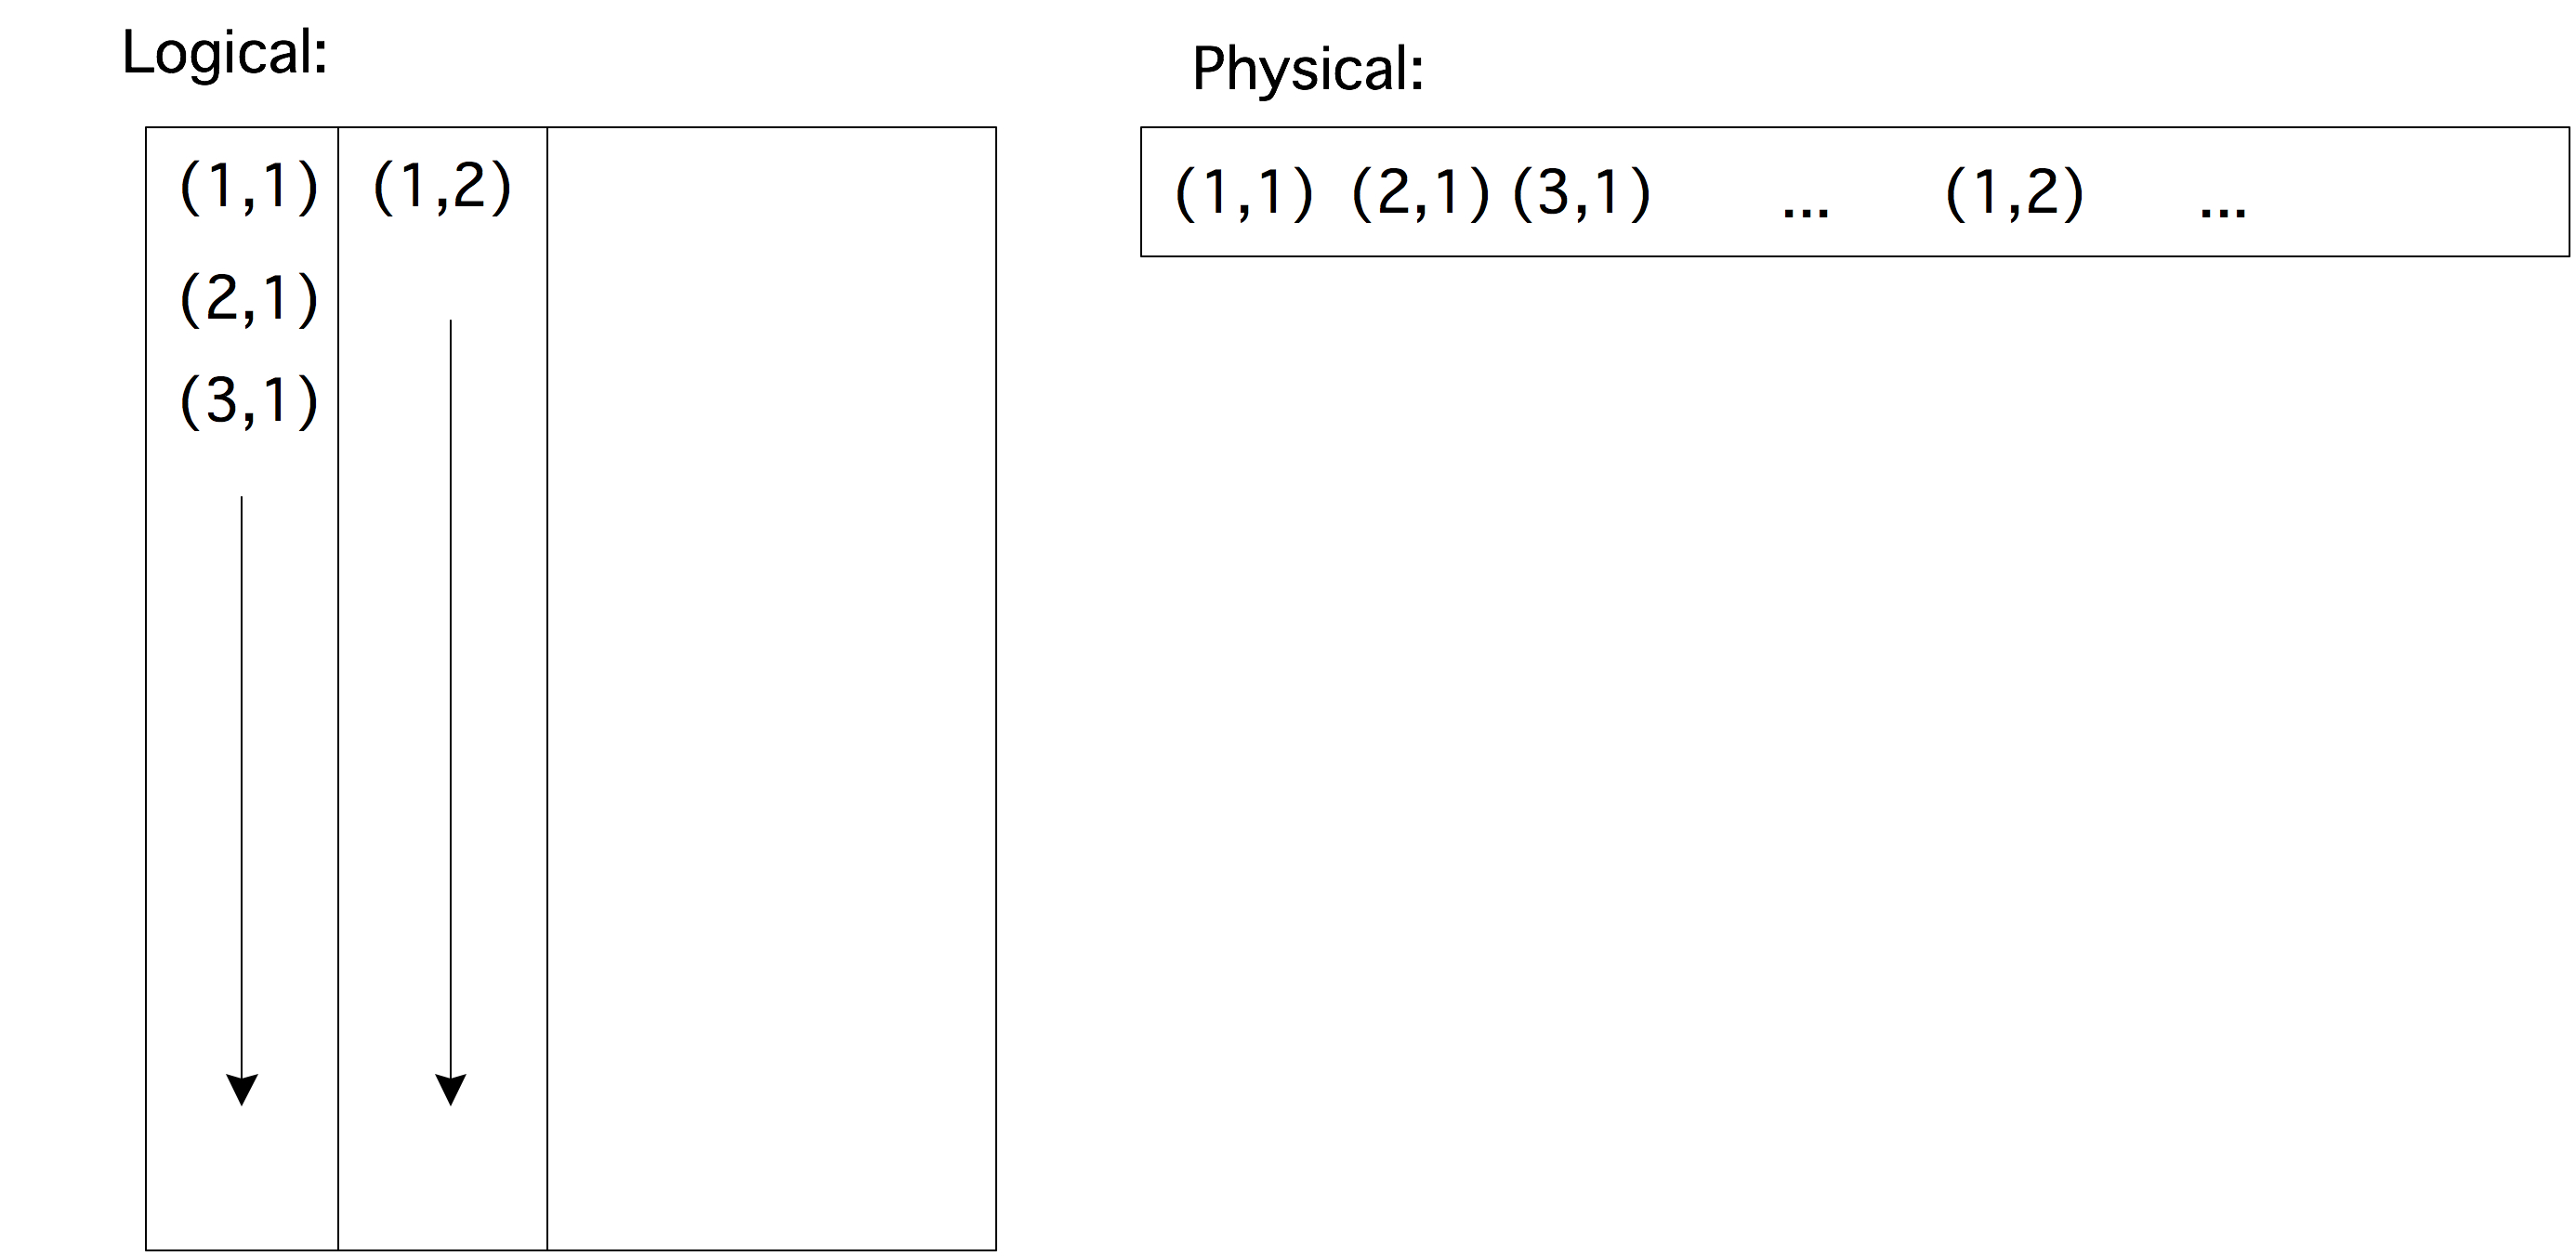
\includegraphics[scale=.14]{densearray}
  \caption{Column-major storage of an array in Fortran.}
  \label{fig:densearray}
\end{figure}
This is also described informally as `the leftmost index varies
quickest'.

Arrays in~C, on the other hand, are laid out in \indexterm{row-major} order.
How to create a C array that can be handled by Blas routines
is discussed in section~\ref{sec:CFarrays}.

\Level 2 {Submatrices and the {\tt LDA} parameter}

Using the storage scheme described above, it is clear how to store an
$m\times n$ matrix in $mn$ memory locations. However, there are many
cases where software needs access to a matrix that is a subblock of
another, larger, matrix. As you see in figure~\ref{fig:lda1}
\begin{figure}[ht]
  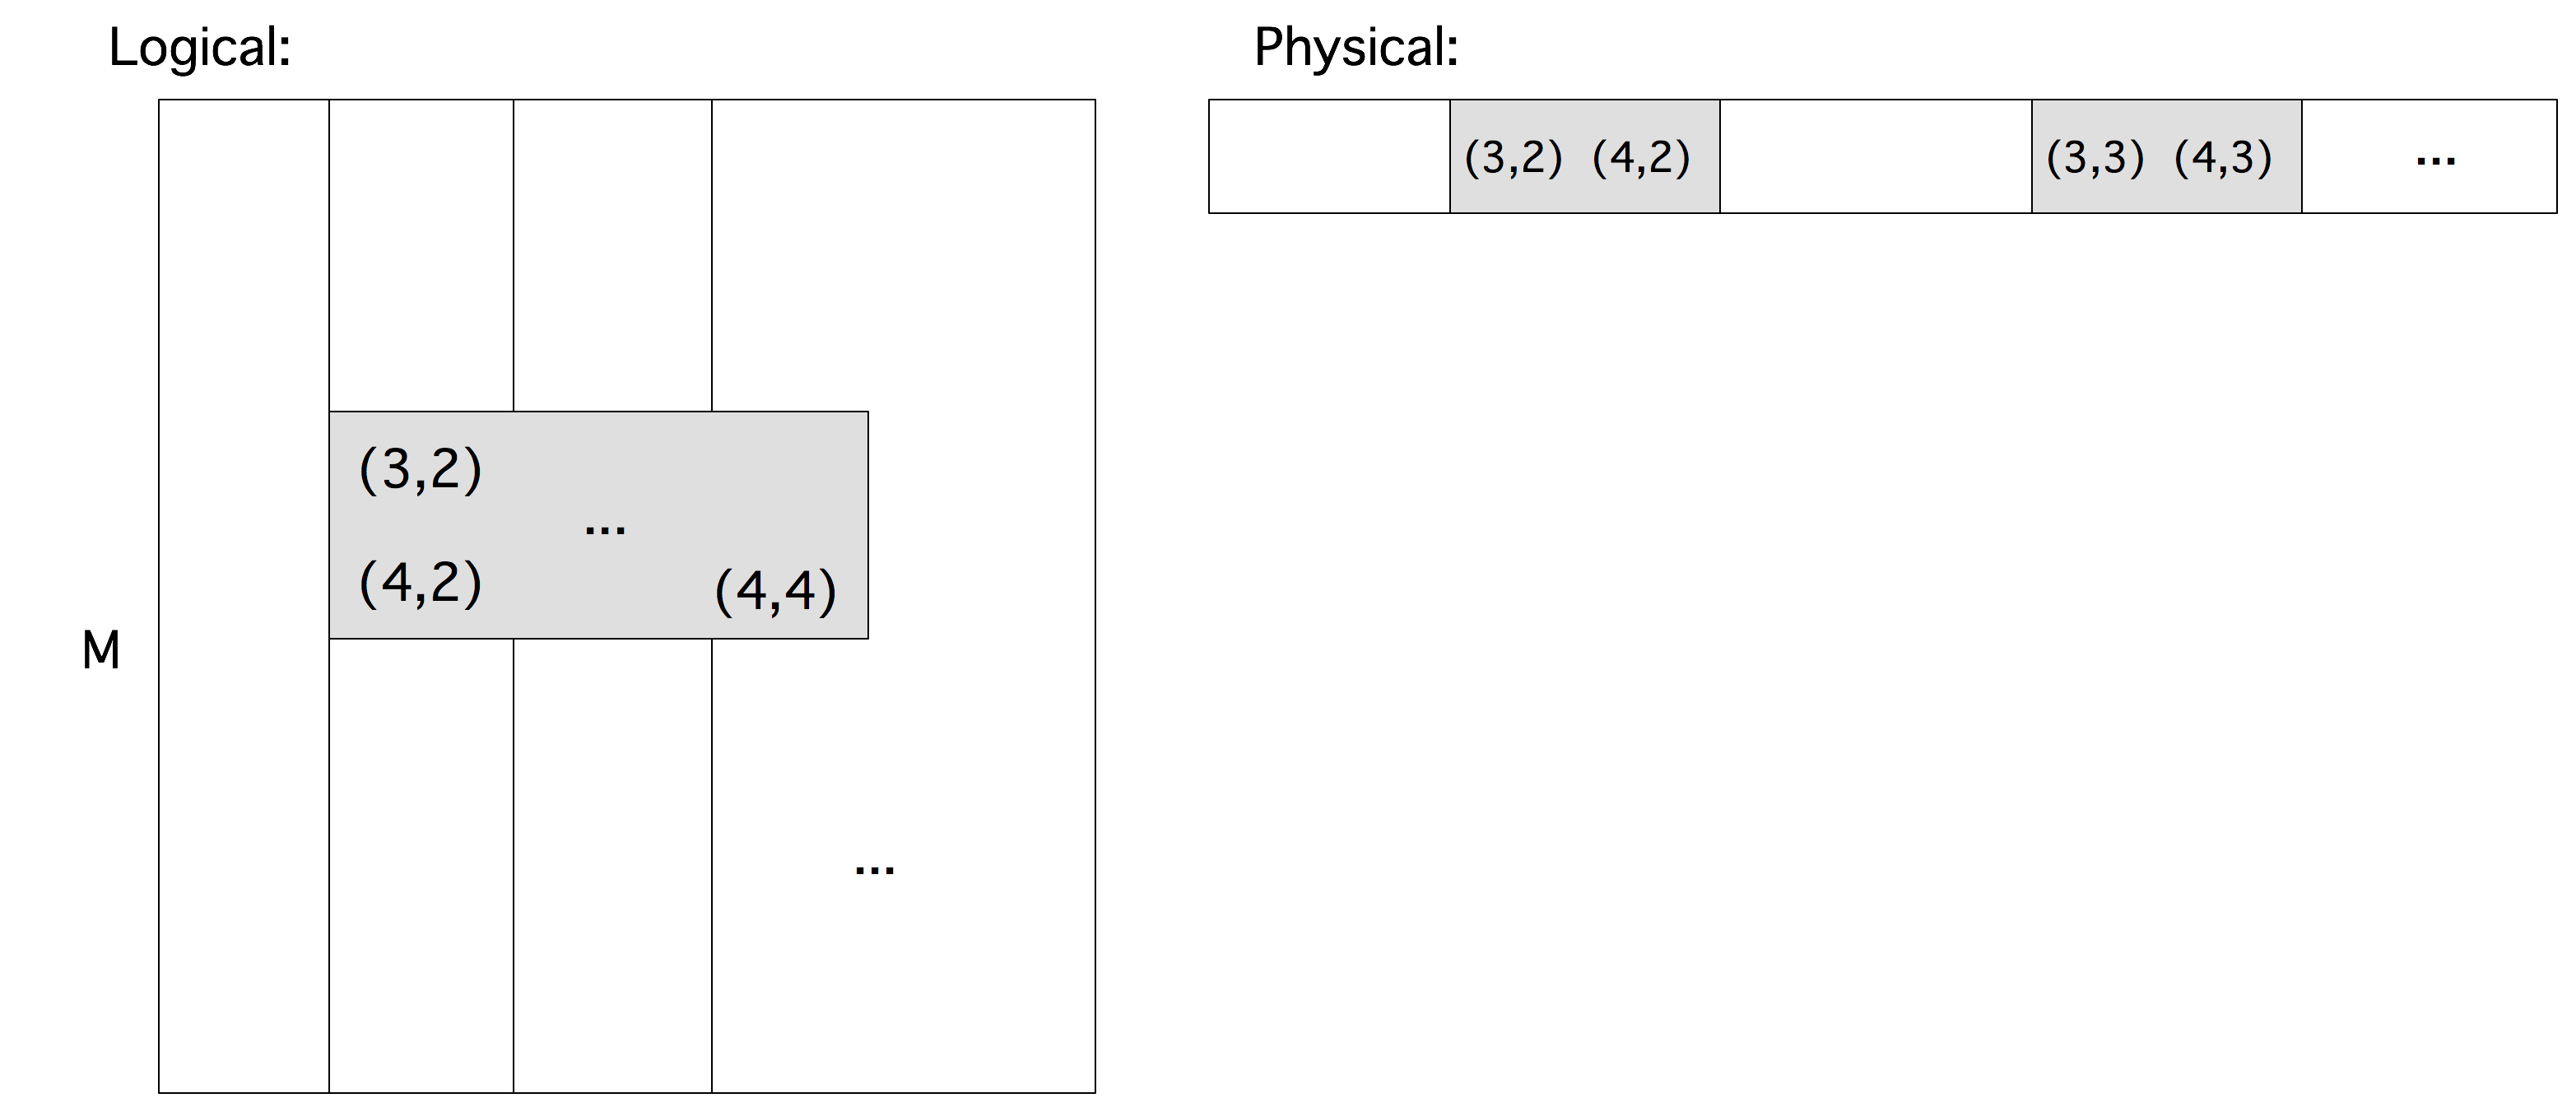
\includegraphics[scale=.14]{denselda}
  \caption{A subblock out of a larger matrix.}
  \label{fig:lda1}
\end{figure}
such a subblock is no longer contiguous in memory. The way to describe
this is by introducing a third parameter in addition to~{\tt M,N}: we
let {\tt LDA} be the `leading dimension of~{\tt A}', that is, the
allocated first dimension of the surrounding array. This is
illustrated in figure~\ref{fig:lda2}.
\begin{figure}
  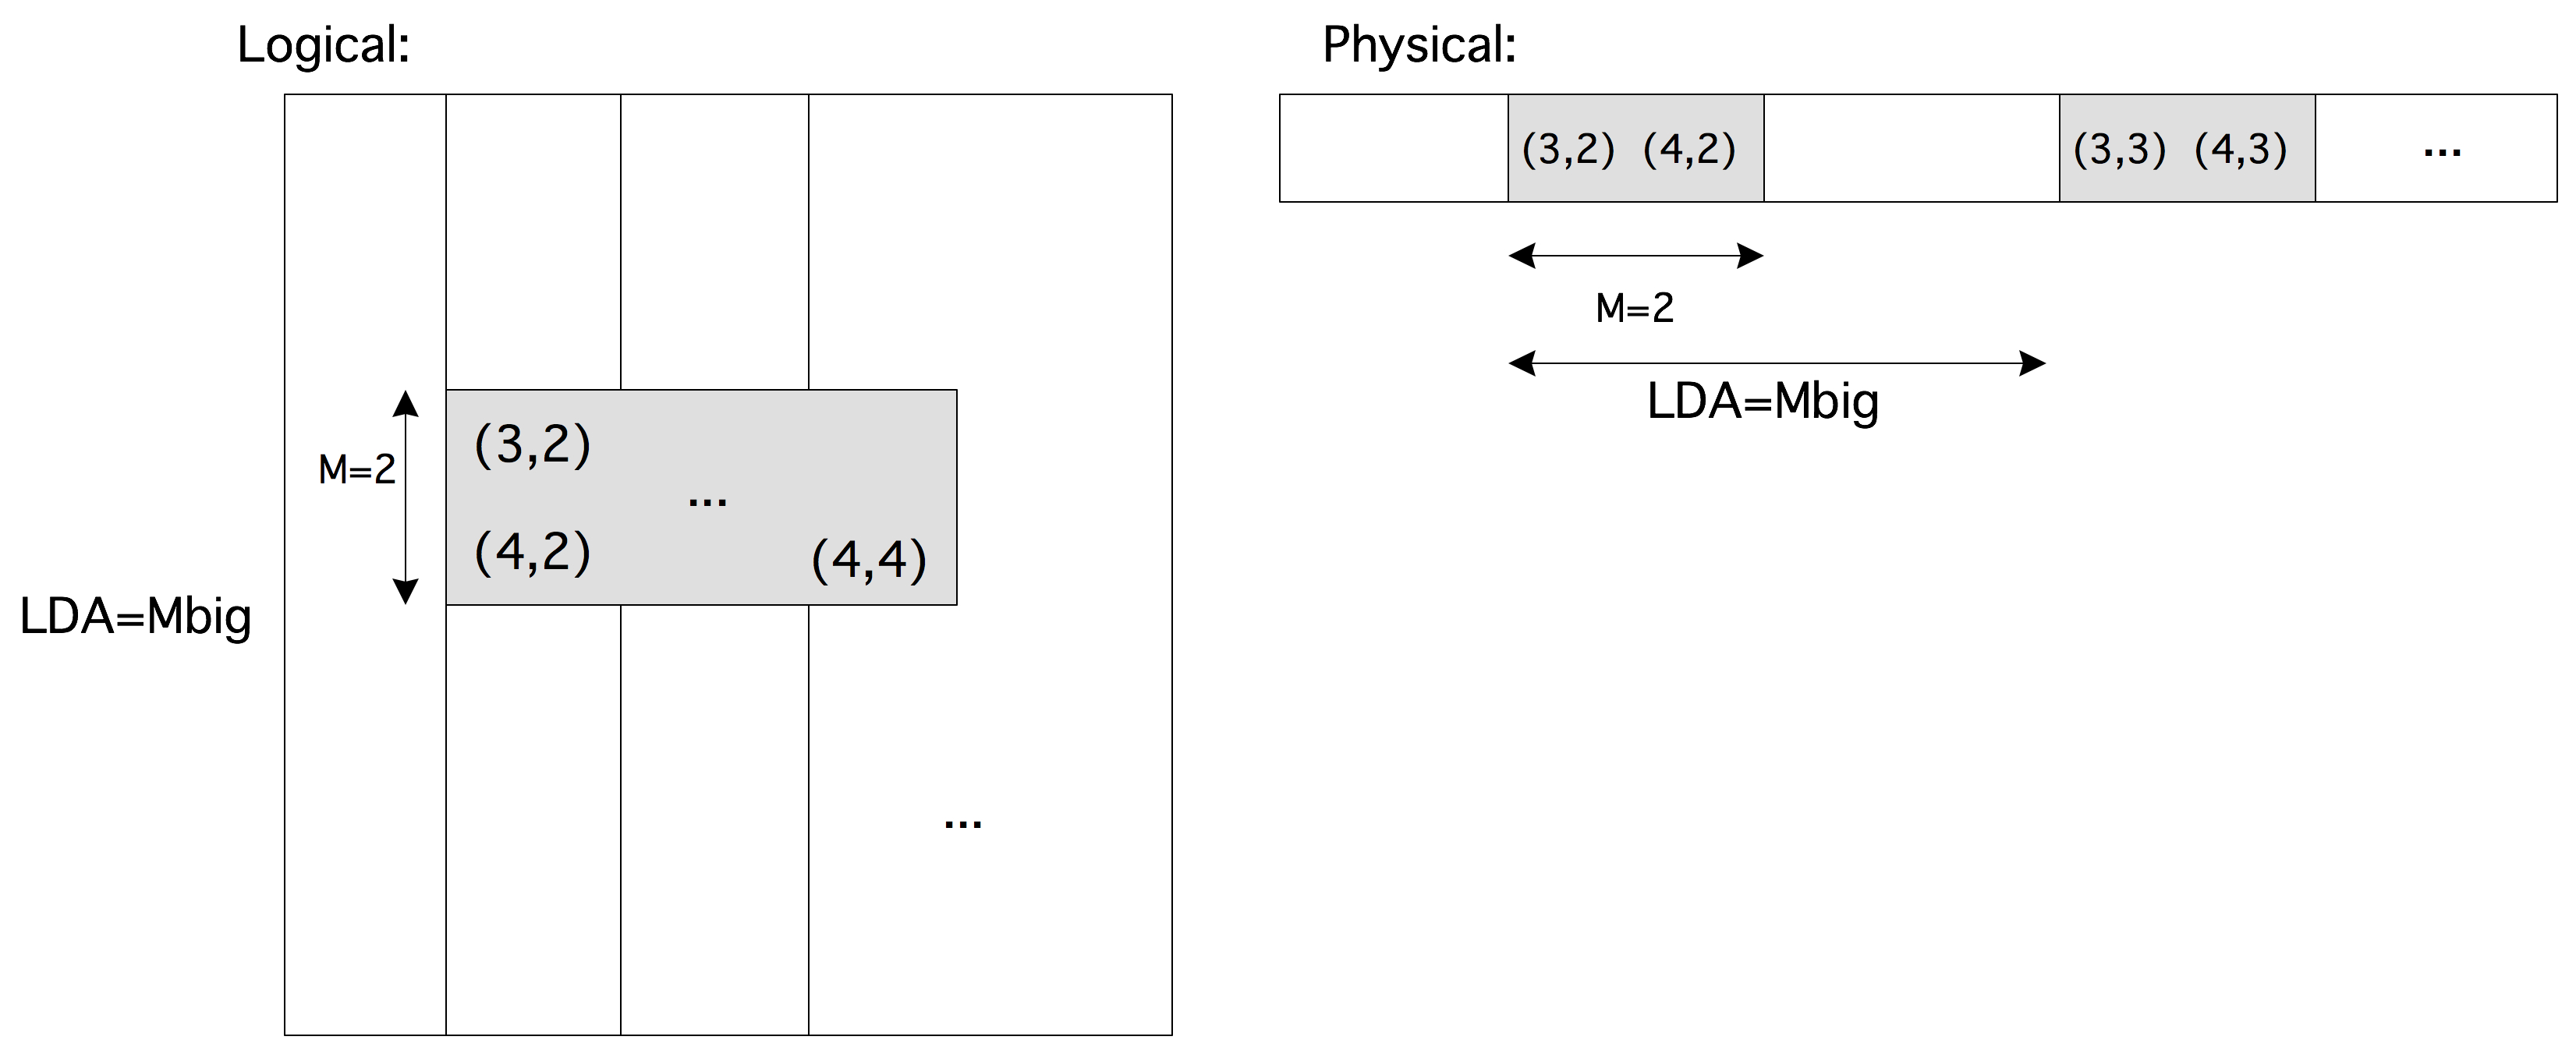
\includegraphics[scale=.14]{denselda2}
  \caption{A subblock out of a larger matrix, using {\tt LDA}.}
  \label{fig:lda2}
\end{figure}
To pass the subblock to a routine, you would specify it as
\begin{verbatim}
call routine( A(3,2), /* M= */ 2, /* N= */ 3, /* LDA= */ Mbig, ... )
\end{verbatim}

\index{BLAS!data format|)}

\Level 1 {Performance issues}

The collection of BLAS and LAPACK routines are a \emph{de facto}
standard: the \ac{API} is fixed, but the implementation is not.
You can find reference implementations on the
\indexterm{netlib} website (\texttt{netlib.org}), but
these will be very low in performance.

On the other hand, many LAPACK routines can be based on
the matrix-matrix product (BLAS routine \texttt{gemm}),
which you saw in section~\HPSCref{sec:goto-gemm} has the potential
for a substantial fraction of peak performance. To achieve
this, you should use an optimized version, such as
\begin{itemize}
\item \indexterm{MKL}, the Intel math-kernel library;
\item OpenBlas (\texttt{http://www.openblas.net/}), an open source
  version of the original \emph{Goto BLAS}\index{matrix-matrix product!Goto implementation}; or
\item \indexterm{blis} (\texttt{https://code.google.com/p/blis/}), a BLAS replacement and
  extension project.
\end{itemize}

\Level 1 {Some simple examples}

Let's look at some simple examples.

The routine \n{xscal} scales a vector in place.
\begin{verbatim}
! Fortran
subroutine dscal(integer N, double precision DA,
    double precision, dimension(*) DX, integer INCX )  
// C
void cblas_dscal (const MKL_INT n, const double a, 
    double *x, const MKL_INT incx);
\end{verbatim}
A simple example:
%
\verbatimsnippet{scale}

The same in~C:
%
\verbatimsnippet{scalecb}

Many routines have an increment parameter. For \n{xscale} that's the final parameter:
%
\verbatimsnippet{scaleinc}

The matrix-vector product \n{xgemv} computes $y\leftarrow \alpha Ax+\beta y$,
rather than $y\leftarrow Ax$.
The specification of the matrix takes the \n{M,N} size parameters,
and a character argument \n{'N'} to indicate that the matrix is not transposed.
Both of the vectors have an increment argument.
\begin{verbatim}
subroutine dgemv(character TRANS,
    integer M,integer N,
    double precision ALPHA,
    double precision, dimension(lda,*) A,integer LDA,
    double precision, dimension(*) X,integer INCX,
    double precision BETA,double precision, dimension(*) Y,integer INCY
    )
\end{verbatim}
An example of the use of this routine:
%
\verbatimsnippet{mvp}

The same example in~C has an extra parameter to indicate whether the matrix
is stored in row or column major storage:
%
\verbatimsnippet{mvpc}



% LocalWords:  Eijkhout PETSc Linpack Eispack Lapack MKL Scalapack YY
% LocalWords:  PLapack mkl cblas dasum CblasNoTrans XYYZZZ ZZZ GE LDA
% LocalWords:  SY UPLO SPOTRF SGBTRF overallocation SPDTRF SVD SV LU
% LocalWords:  DGESV SVX xGELS QR LQ xGELSY xGELSS xGELSD LSE GLM xSY
% LocalWords:  xHE SP SB EV EVX EVD EVR xGE Schur ES ESX SDD GV GVX
% LocalWords:  GVD Nonsymmetric GGES GGESX eigen GGEV GGEVX svd GGSVD
% LocalWords:  Submatrices subblock de API netlib website org gemm
% LocalWords:  OpenBlas blis xscal scalecb xscale scaleinc xgemv mvp
% LocalWords:  mvpc
